\chapter{Brugermanual}

\begin{figure}[ht]
\begin{minipage}[b]{0.5\linewidth}
\centering
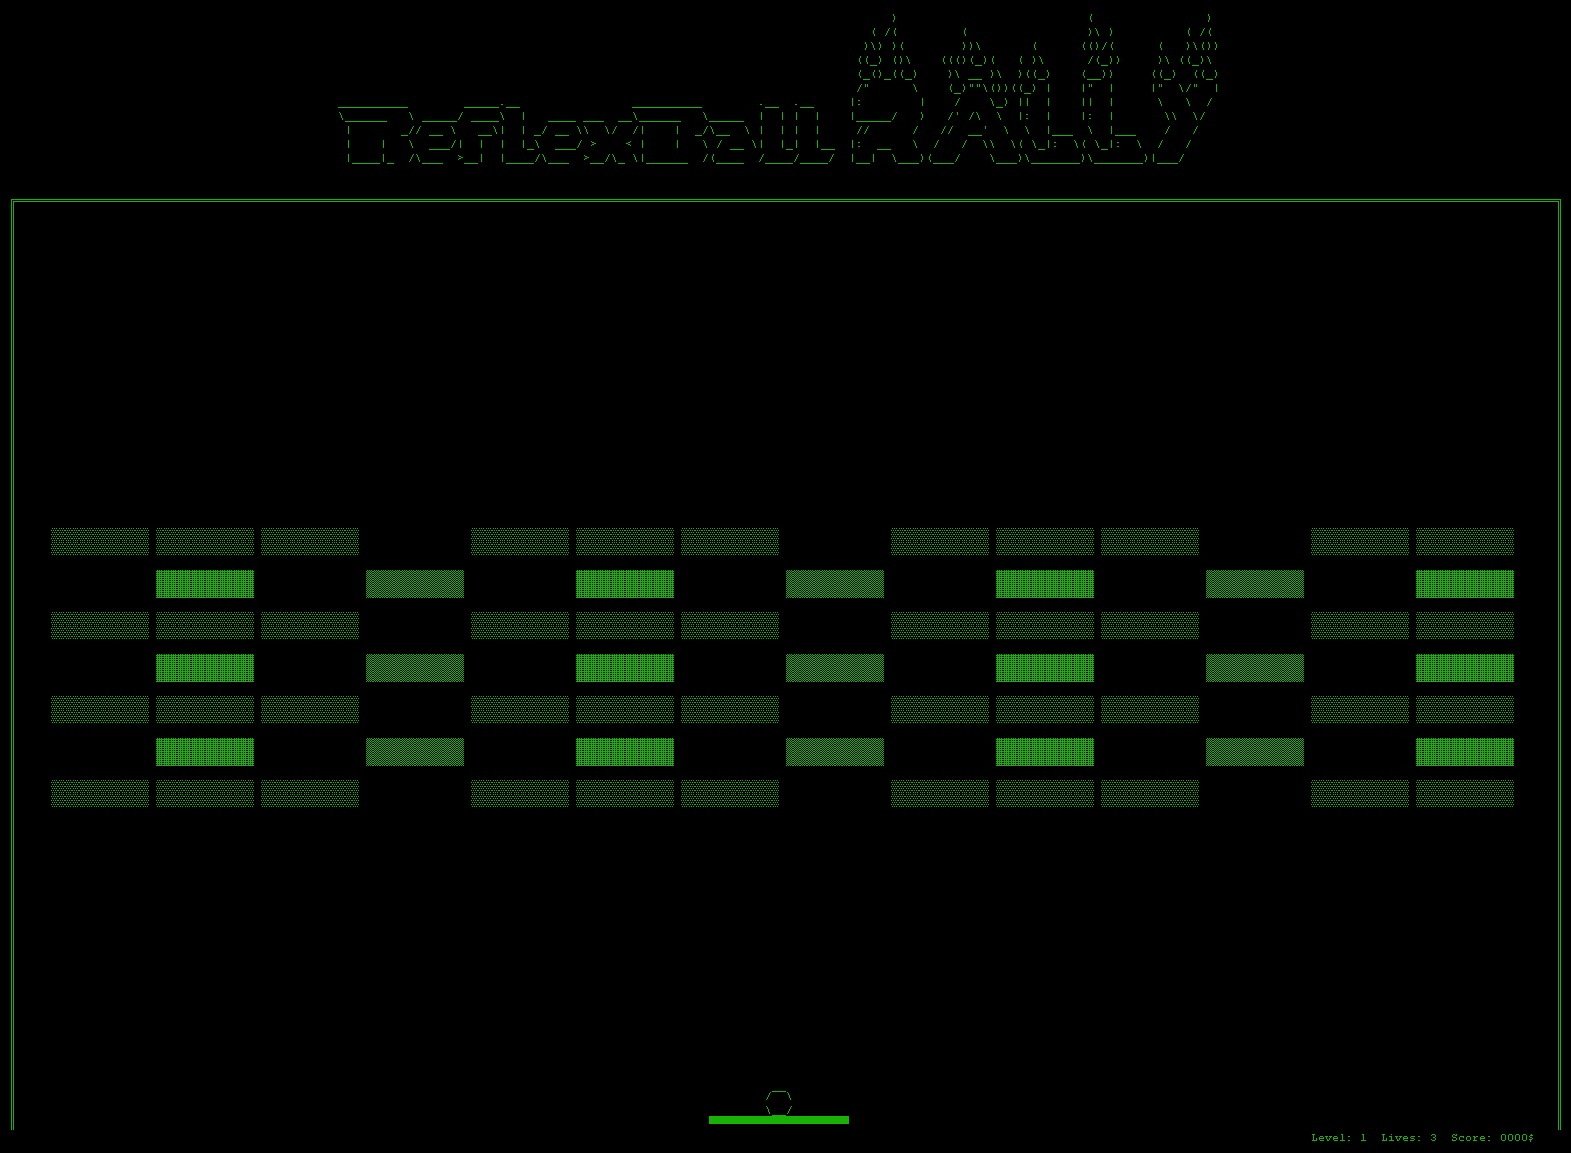
\includegraphics[scale=0.12]{figs/screenshots/level1.png}
\caption{Level 1}
\label{fig:level1}
\end{minipage}
\hspace{0.5cm}
\begin{minipage}[b]{0.5\linewidth}
\centering
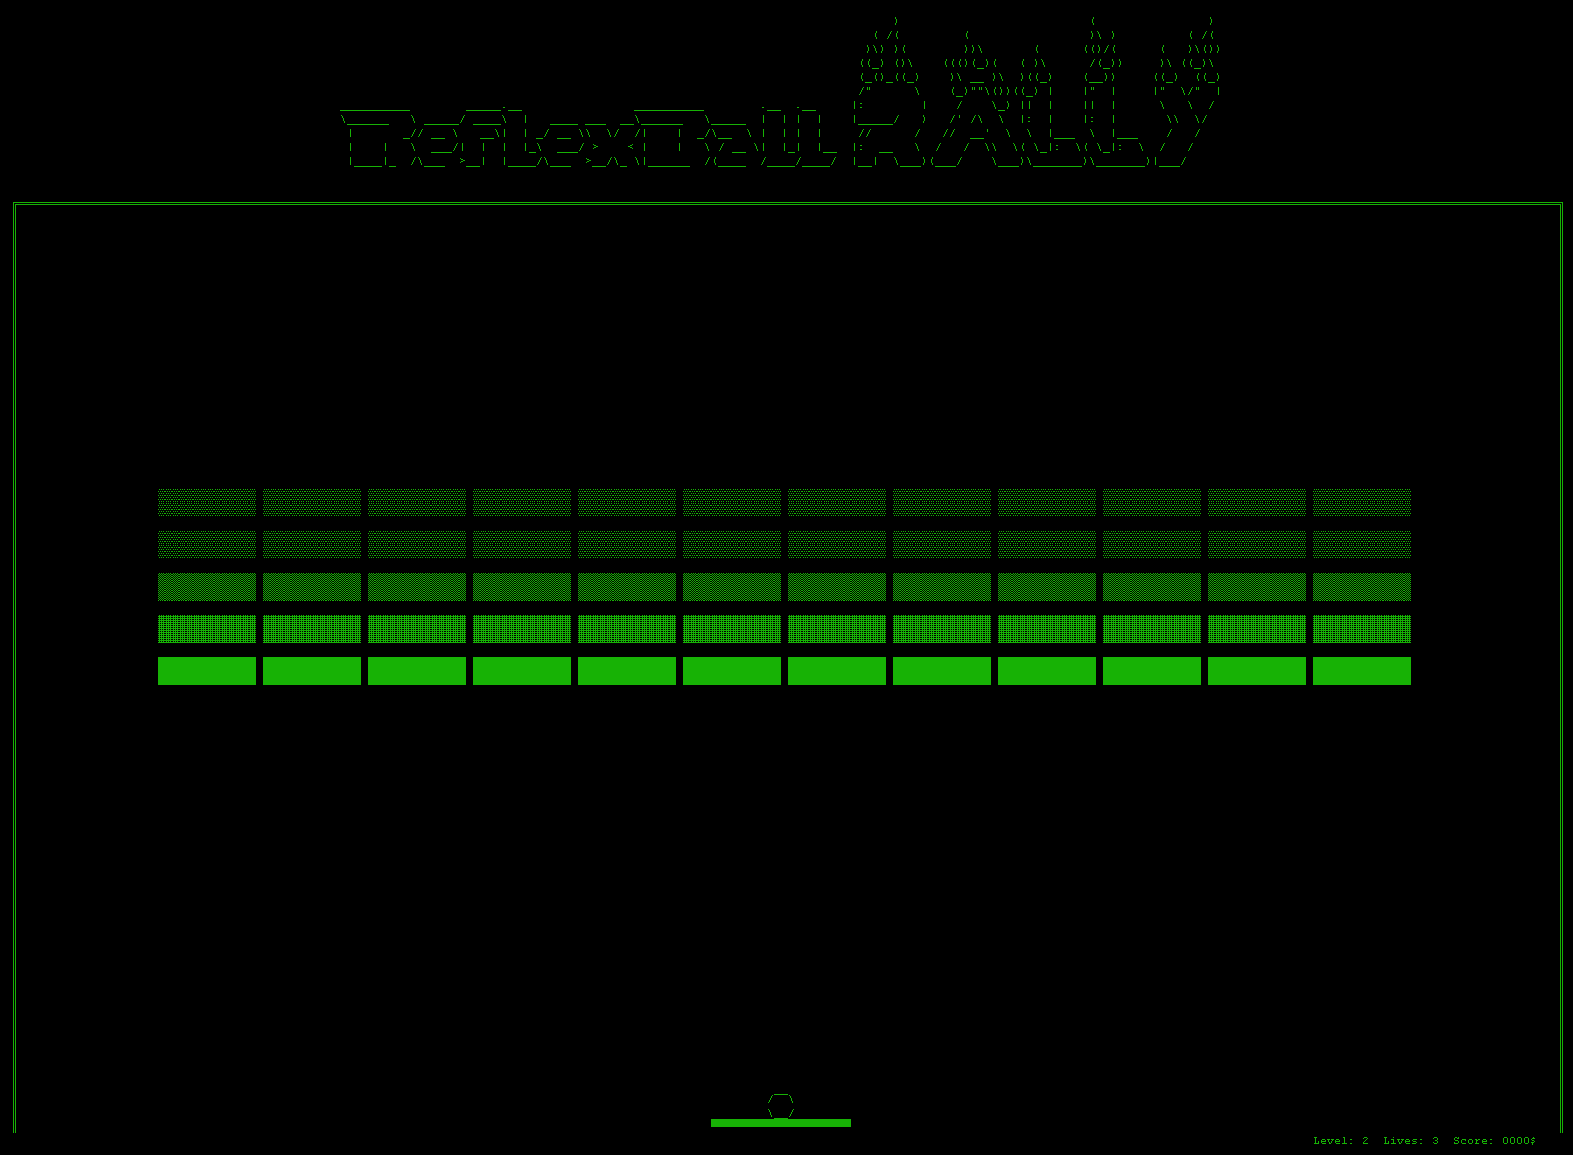
\includegraphics[scale=0.12]{figs/screenshots/level2.png}
\caption{Level 2}
\label{fig:level2}
\end{minipage}
\end{figure}

\begin{figure}[ht]
\begin{minipage}[b]{0.5\linewidth}
\centering
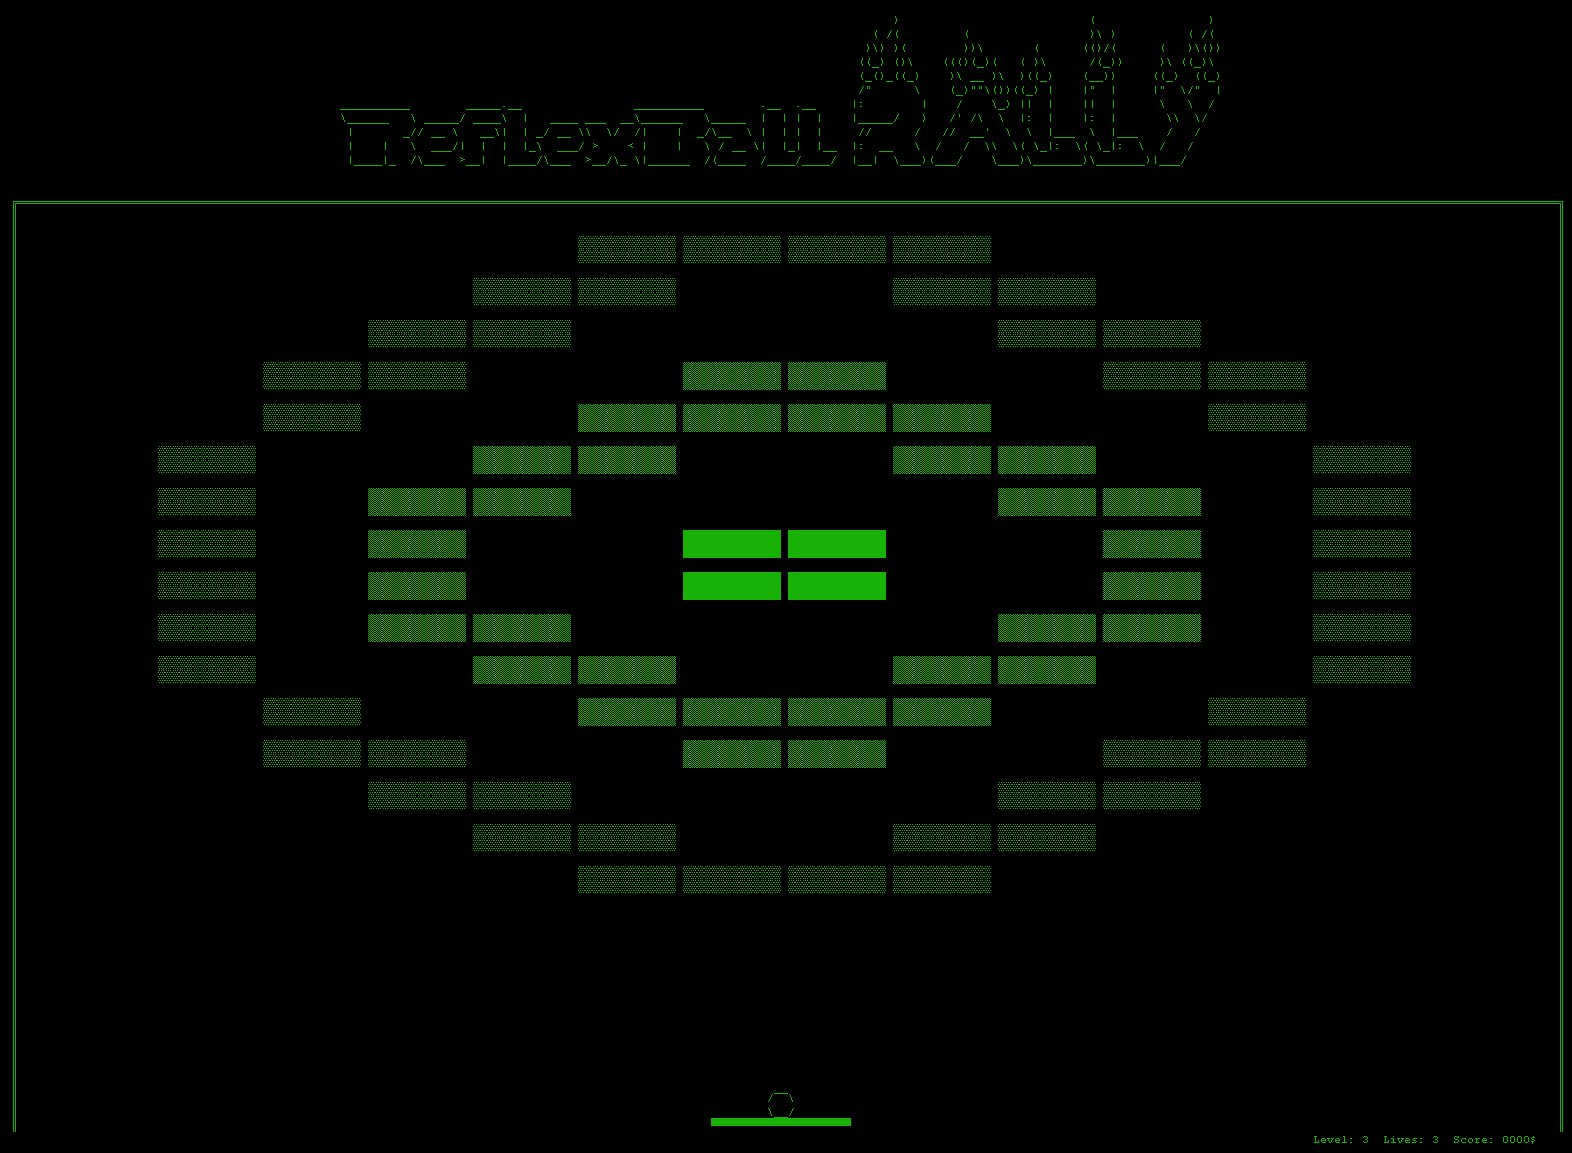
\includegraphics[scale=0.12]{figs/screenshots/level3.png}
\caption{Level 3}
\label{fig:level3}
\end{minipage}
\hspace{0.5cm}
\begin{minipage}[b]{0.5\linewidth}
\centering
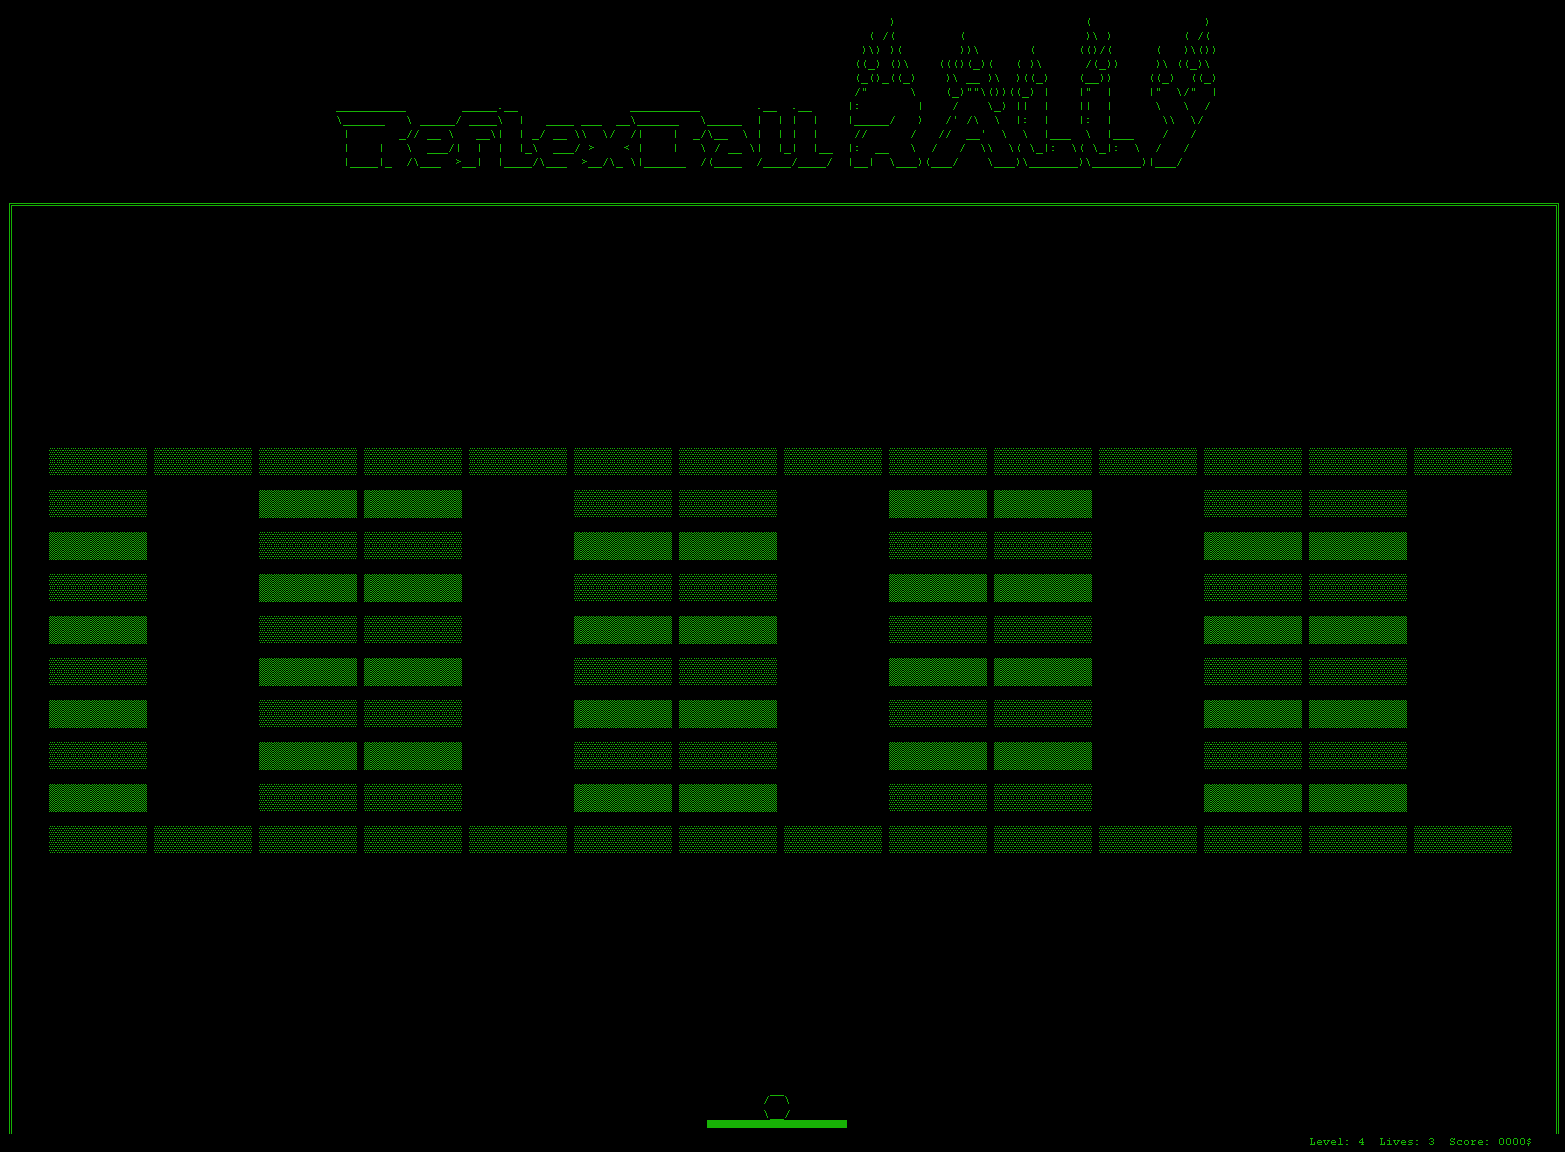
\includegraphics[scale=0.12]{figs/screenshots/level4.png}
\caption{Level 4}
\label{fig:level4}
\end{minipage}
\end{figure}

\begin{figure}[ht]
\begin{minipage}[b]{0.5\linewidth}
\centering
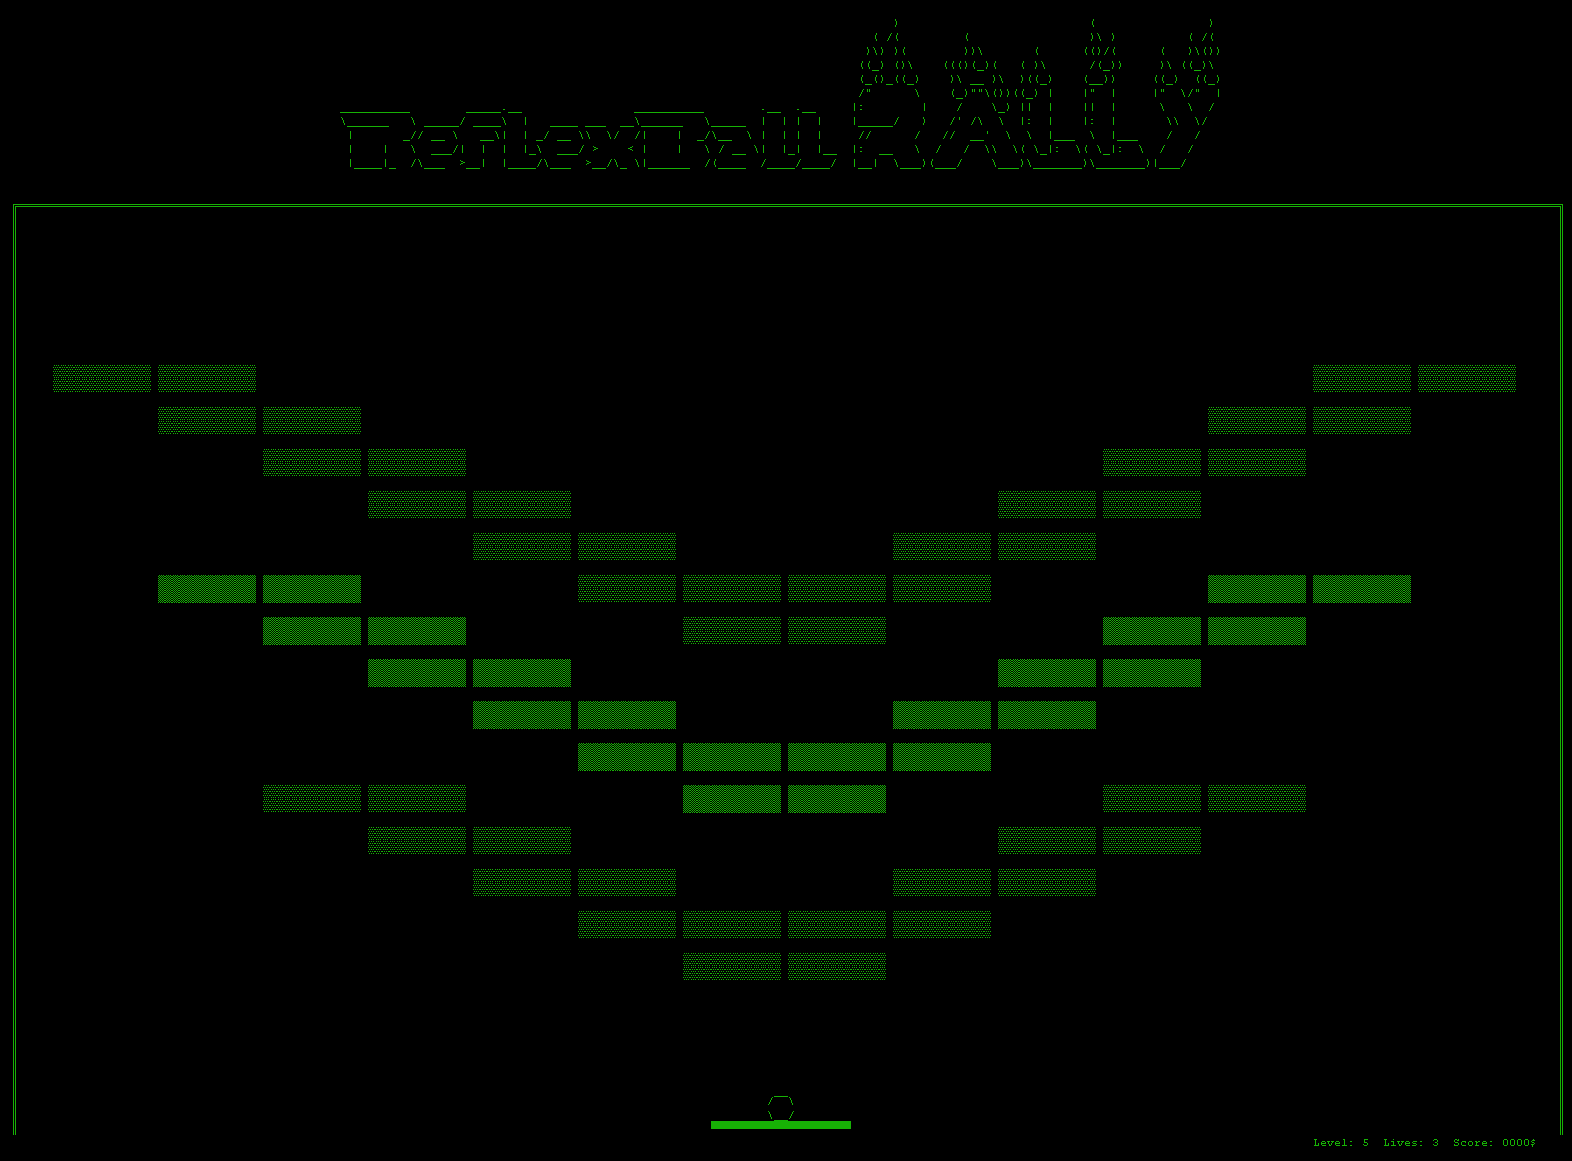
\includegraphics[scale=0.12]{figs/screenshots/level5.png}
\caption{Level 5}
\label{fig:level5}
\end{minipage}
\hspace{0.5cm}
\begin{minipage}[b]{0.5\linewidth}
\centering
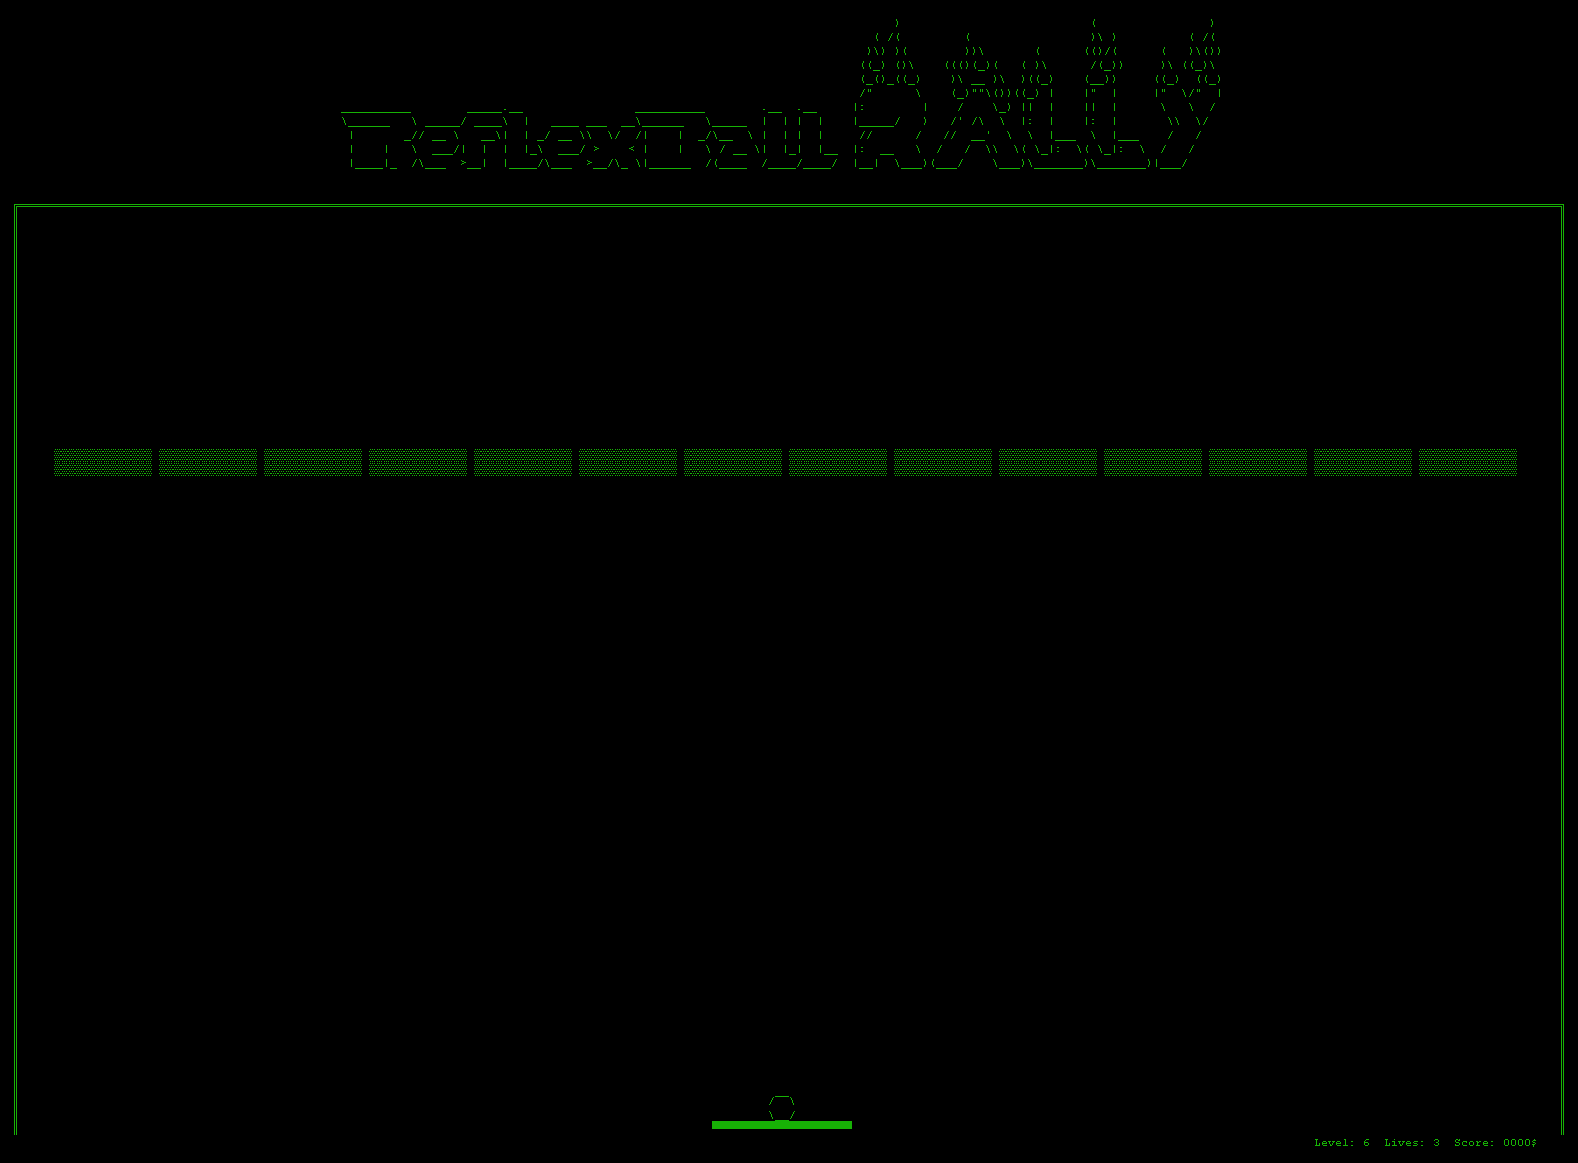
\includegraphics[scale=0.12]{figs/screenshots/level6.png}
\caption{Level 6}
\label{fig:level6}
\end{minipage}
\end{figure}